\documentclass[12pt]{article}
\usepackage{../lecture}
\lecture{18}{BFS and Dijkstra's Algorithm}
\date{March 30, 2021}

\begin{document}
\maketitle

\section{Breadth First Search}
\subsection{Overview}
\begin{itemize}
    \item BFS is obtained from BasicSearch by processing edges using a data structure called a queue.
    \item It processes the vertices in the graph in the order of their shortest distance from the vertex $s$ (the start vertex).
    \item While DFS is good for exploring graph strcture, BFS is good for exploring distances.
    \item In a queue, elements are extracted in first-in first-out (FIFO) order. It supports the following operations:
    \begin{itemize}
        \item \texttt{enqueue}: Adds an element to the end of the list.
        \item \texttt{dequeue}: Removes an element from the front of the list.
    \end{itemize}
\end{itemize}

\subsection{BFS Algorithm}
\begin{itemize}
    \item Given a (directed or undirected) graph $G = (V, E)$ and node $s \in V$, running in $O(m + n)$
    \item[] \lstinputlisting{code/bfs.sudo}
    \begin{center}
        \item[] 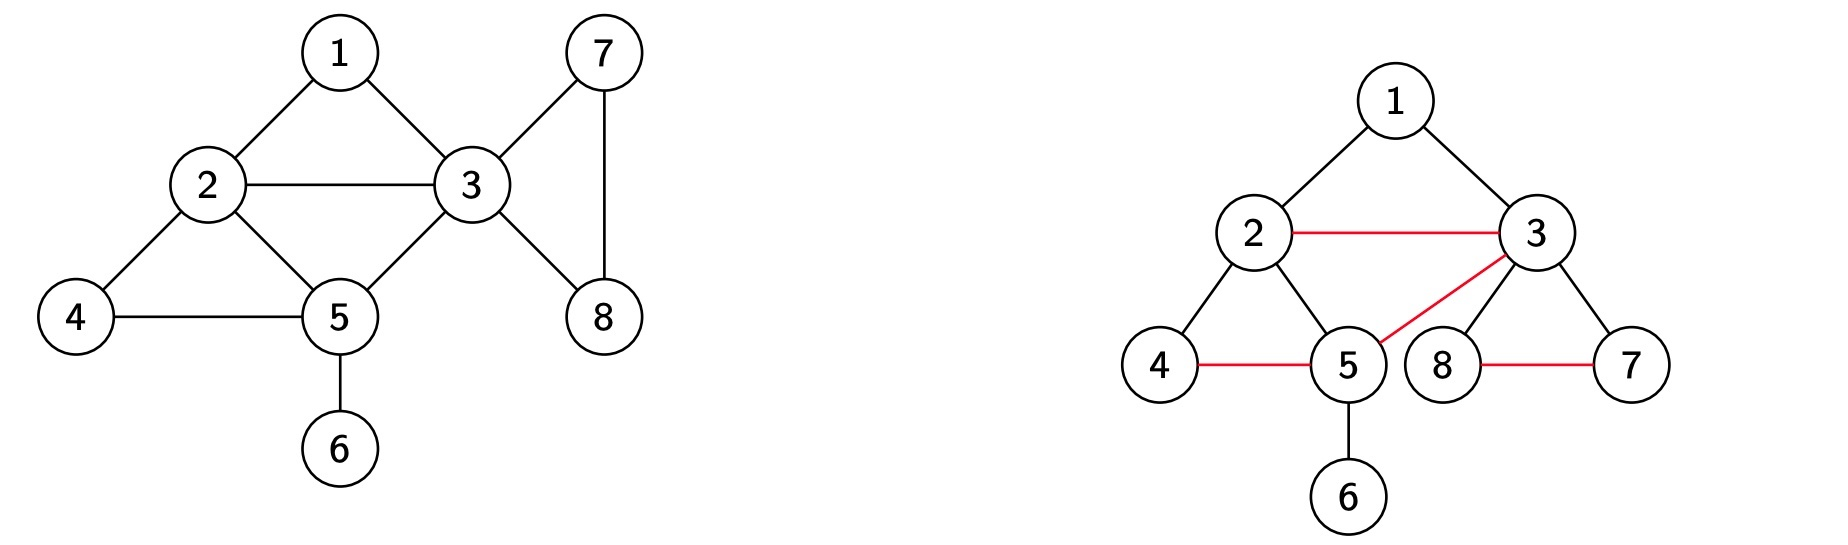
\includegraphics[width=0.8\textwidth]{images/bfs-undirected-example.jpg}
    \end{center}
    \item The BFS tree is te set of black edges.
    \item We can also keep track of distance from $s$ to each node in BFS.
    \item[] \lstinputlisting{code/bfs-distance.sudo}
\end{itemize}

\subsection{Properties of BFS on Undirected Graphs}
\begin{itemize}
    \item The following properties hold upon termination of \texttt{BFS(s)}.
    \item The search tree contains exactly the set of vertices in the connected component of $s$.
    \item If $dist(u) < dist(v)$, then $u$ is visited before $v$.
    \item For every vertex $u$, $dist(u)$ is the length of the shortest path from $s$ to $u$.
    \item If $u$ is reachable from $s$ and $\{ u, v \} \in E$, then $\left|dist(v) - dist(u)\right| \leq 1$.
\end{itemize}

\subsection{Properties of BFS on Directed Graphs}
\begin{itemize}
    \item The following properties hold upon termination of \texttt{BFS(s)}.
    \item The search tree contains exactly the set of vertices reachable from $s$.
    \item If $dist(u) < dist(v)$, then $u$ is visited before $v$.
    \item For every vertex $u$, $dist(u)$ is the length of the shortest path from $s$ to $u$.
    \item If $u$ is reachable from $s$ and $(u, v) \in E$, then $dist(v) - dist(u) \leq 1$. However, it is not necessarily the case that $dist(u) - dist(v) \leq 1$.
    \item[] 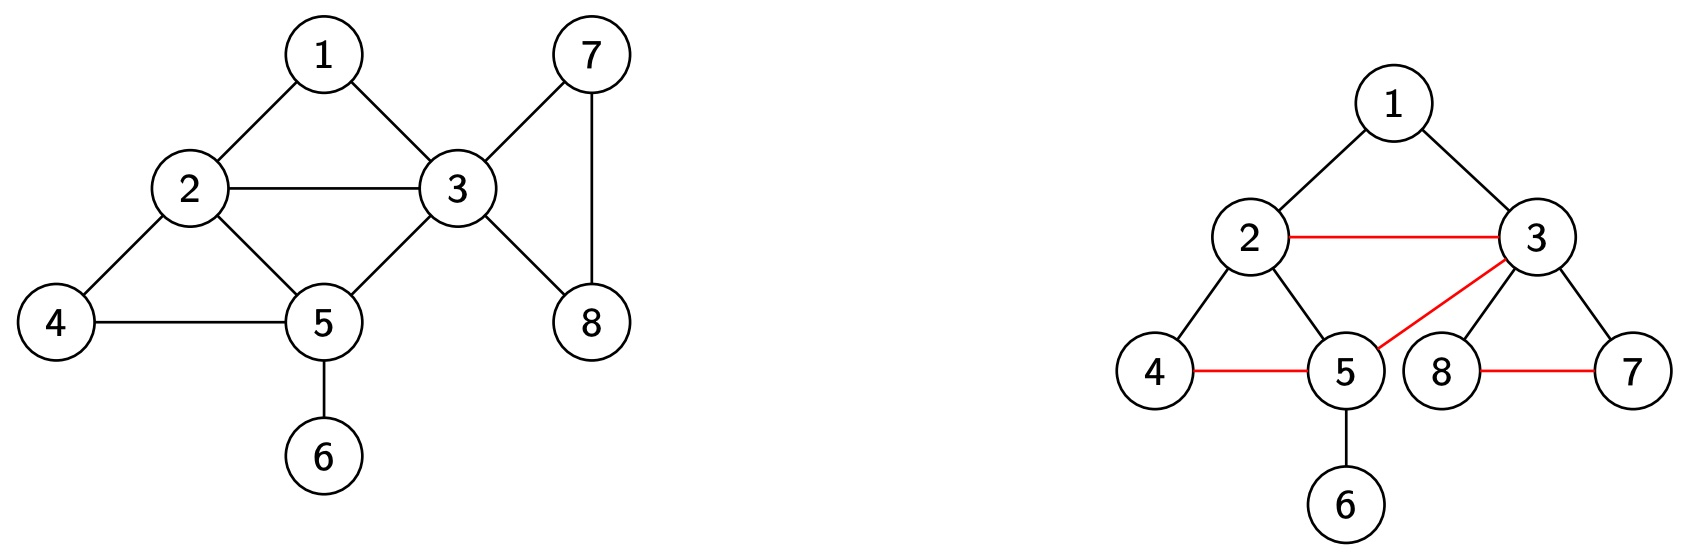
\includegraphics[width=\textwidth]{images/bfs-undirected--layers-example.jpg}
\end{itemize}

\section{Shortest Paths and Dijkstra's Algorithm}

\subsection{Shortest Path Problems}
\begin{itemize}
    \item \textit{Input} A (directed or undirected) graph $G = (V, E)$ with edge lengths (or costs). For edge $e = (u, v)$, $l(e) = l(u, v)$ is its length.
    \item Given nodes $s, t$, find a shortest path from $s$ to $t$.
    \item Given node $s$, find a shortest from $s$ to all other nodes.
    \item Find shortest paths for all pairs of nodes.
    \item We can restrict our attention to directed graphs, as undirected graph problems can be reduced to directed graph problems.
\end{itemize}

\subsection{Single Source Shortest Paths}
\begin{itemize}
    \item \textit{Special case}: All edge lengths are $1$.
    \begin{itemize}
        \item Run \texttt{BFS(s)} to get shortest path distances from $s$ to all other nodes.
        \item This is an $O(m + n)$ time algorithm.
    \end{itemize}
    \item \textit{Special case}: $l(e)$ is an integer for all $e$.
    \begin{itemize}
        \item We can reduce the graph to unit edge length p
        \item Let $L = max_e l(e)$. The new graph has $O(mL)$ edges and $O(mL + n)$ nodes. BFS would take $O(mL + n)$ time. This is not efficient if $L$ is large enough.
    \end{itemize}
    \item BFS works because \texttt{BFS(s)} explores nodes in increasing distance from $s$.
    \begin{itemize}
        \item Let $G$ be a directed graph with non-negative edge lengths. Let $dist(s, v)$ denote the shortest path length from $s$ to $v$. If $s = v_0 \rightarrow v_1 \rightarrow ... \rightarrow v_k$ is a shortest path from $s$ to $v_k$, then for $1 \leq i < k$
        \begin{itemize}
            \item $s = v_0 \rightarrow v_1 \rightarrow ... \rightarrow v_i$ is a shortest path from $s$ to $v_i$.
            \item $dist(s, v_i) \leq dist(s, v_k)$.
        \end{itemize}
    \end{itemize}
    \item A basic strategy is exploring vertices in increasing order of distance from $s$:
    \item[] \lstinputlisting{code/basic-strategy.sudo}
\end{itemize}

\subsection{Finding the $i$th Closest Node}
\begin{itemize}
    \item $X$ contains the $i - 1$ closest nodes to $s$. Next we need to find the $i$th closest node from $V - X$.
    \item The $i$th closest node is adjacent to $X$.
    \begin{itemize}
        \item Let $P$ be a shortest path from $s$ to $v$ where $v$ is the $i$th closest node. Then, all intermediate nodes in $p$ belong to $X$.
        \item If $P$ had an intermediate node $u$ not in $X$, then $u$ would be closer to $s$ than $v$. That would imply $v$ is not the $i$th closest node to $s$ -- recall that $X$ already has the $i - 1$ closest nodes.
    \end{itemize}
    \item For each $u \in V - X$, let $P(s, u, X)$ be a shortest path from $s$ to $u$ using only nodes in $X$ as intermediate vertices.
    \item Let $d'(s, u)$ be the length of $P(s, u, X)$.
    \item For each $u \in V - X$, we can observe that
    \begin{itemize}
        \item $dist(s, u) \leq d'(s, u)$ since we are constraining the paths by only usings nodes in $X$ in $d'$.
        \item $d'(s, u) = min_{t \in x}(dist(s, t) + l(t, u))$
    \end{itemize}
    \item If $v$ is the $i$th closest node to $s$, then $d'(s, v) = dist(s, v)$.
    \begin{itemize}
        \item Let $v$ be the $i$th closest node to $s$. Then there is a shortest path $P$ from $s$ to $v$ that contains only nodes in $X$ as intermediate nodes. Therefore $d'(s, v) = dist(s, v)$.
    \end{itemize}
    \item The $i$th closest node to $s$ is the node $v \in V - X$ such that $d'(s, v) = min_{u \in V - X}d'(s, u)$.
    \begin{itemize}
        \item For every node $u \in V - X$, $dist(s, u) \leq d'(s, u)$ and for the $i$th closest node $v$, $dist(s, v) = d'(s, v)$. Moreover, $dist(s, u) \geq dist(s, v)$ for each $u \in V - X$.
    \end{itemize}
    \item This gives us the following algorithm:
    \item[] \lstinputlisting{code/single-source-shortest-path.sudo}
    \item The algorithm runs in $O(n(m + n))$ time.
    \begin{itemize}
        \item There are $n$ outer iterations. In each iteration, computing $d'(s, u)$ for each $u$ by scanning all edges out of nodes in $X$ takes $O(m + n)$ time.
        \item The main work is to compute the $d'(s, u)$ values in each iteration.
        \item $d'(s, u)$ changes from iteration $i$ to $i + 1$ only because of the node $v$ that is added to $X$ in iteration $i$.
    \end{itemize}
    \item We can create an improved algorithm that runs in $O(m + n^2)$ time.
    \begin{itemize}
        \item $n$ outer iterations and in each iteration
        \begin{itemize}
            \item updating $d'(s, u)$ after $v$ is added takes $O(deg(v))$ time so total work is $O(m)$, since a node enters $X$ only once.
            \item finding $v$ from $d'(s, u)$ values is $O(n)$ time.
        \end{itemize}
    \end{itemize}
\end{itemize}

\subsection{Dijkstra's Algorithm}
\begin{itemize}
    \item We eliminate $d'(s, u)$ and let $dist(s, u)$ maintain it instead.
    \item We update $dist$ values after adding $v$ by scanning edges out of $v$.
    \item[] \lstinputlisting{code/dijkstra.sudo}
    \item We can use priority queues to maintain dist values for fast running times.
    \begin{itemize}
        \item Using heaps and standard priority queues gives us a running time of $O(\log n(m + n))$.
    \end{itemize}
    \item[] \lstinputlisting{code/dijkstra-priority-queue.sudo}
    \begin{itemize}
        \item Using heaps, operations are
        \begin{itemize}
            \item $O(n)$ \texttt{insert}
            \item $O(n)$ \texttt{extractMin}
            \item $O(m)$ \texttt{decreaseKey}
        \end{itemize}
        \item Using fibonacci heaps, operations are
        \begin{itemize}
            \item \texttt{extractMin}, \texttt{insert}, \texttt{delete}, \texttt{meld} in $O(\log n)$ time.
            \item \texttt{decreaseKey} in $O(1)$ in amortized: $l$ \texttt{decreaseKey} operations for $l \geq n$ take together $O(l)$ time.
            \item Relaxed heaps: \texttt{decreaseKey} in $O(1)$ worst case time but at the expense of \texttt{meld} (not necessary for Dijkstra).
        \end{itemize}
    \end{itemize}
    \item Dijkstra's algorithm can be implemented in $O(n\log n + m)$ time. If $m = \Omega(n\log n)$, the running time is linear in input size.
    \item We can also figure out the shortest paths.
    \item[] \lstinputlisting{code/dijkstra-path.sudo}
    \item The edge set $(u, prev(u))$ is the reverse of a shortest path tree rooted at $s$. For each $u$, the reverse of the path from $u$ to $s$ in the tree is a shortest path from $s$ to $u$.
    \begin{itemize}
        \item The edge set $\{ (u, prev(u)) \mid u \in V \}$ induces a directed in-tree rooted at $s$.
    \end{itemize}
    \item Dijkstra's algorithm gives shortest paths from $s$ to all nodes in $V$. To find the shortest paths from all $V$ to $s$
    \begin{itemize}
        \item in undirected graphs, it is the same path as $s$ to $V$, so there is no need to distinguish.
        \item in directed graphs, use Dijkstra's algorithm on $G^{rev}$.
    \end{itemize}
\end{itemize}

\end{document} 
